% \IUref{IUAdmPS}{Administrar Planta de Selección}
% \IUref{IUModPS}{Modificar Planta de Selección}
% \IUref{IUEliPS}{Eliminar Planta de Selección}

%-------------------------------------- TERMINA descripción del caso de uso.

%\begin{UseCase}[archivo de imágen]{UCX}{Nombre del Caso de uso}{
	\begin{UseCase}{CU10.0}{Desactivar área}{
		Esta sección es diferente a la de eliminar áreas, ya que el propósito de éste módulo consiste en desactivar temporalmente un área que no tenga actividad por el momento, no será eliminada permanentemente si no que ya no aparecerá en las áreas registradas, hasta que vuelva a ser activada.
	}
		\UCitem{Versión}{1.0}
		\UCitem{Actor}{Gerente}
		\UCitem{Propósito}{Que se pueda cambiar el estado activo de un área en caso de que existan modificaciones en el uso.}
		\UCitem{Entradas}{Nombre del Área, lista desplegable con las áreas.}
		\UCitem{Origen}{Los datos serán seleccionados  mouse.}
		\UCitem{Salidas}{Mensaje de que el área ha sido desactivada.}
		\UCitem{Destino}{El estado del área se verá reflejado en la base de datos. 
El área no podrá ser mostrada en el área de consultas.}
		\UCitem{Precondiciones}{Que el área se encuentre registrada previamente.
El administrador es el único usuario que puede dar de baja un área.}
		\UCitem{Postcondiciones}{El área registrada se verá reflejada en la sección de consultas.}
		\UCitem{Errores}{Que el sistema no efectué la operación requerida.}
		\UCitem{Tipo}{Caso de uso primario.}
		\UCitem{Observaciones}{}
		\UCitem{Autor}{Francisco García Enríquez.}
		\UCitem{Revisor}{Martin Carrillo.}
	\end{UseCase}

\begin{UCtrayectoria}{Principal}
		\UCpaso[\UCactor] Selecciona del menú principal la opción Áreas.
		\UCpaso Muestra las opciones que el gerente pueda realizar: Registrar Áreas, Consultar Áreas, Eliminar Áreas, Desactivar Áreas y Actualizar Áreas.
		\UCpaso[\UCactor] Selecciona la opción desactivar áreas.
		\UCpaso Carga en una lista desplegable las áreas disponible registradas.
		\UCpaso[\UCactor] Selecciona de la lista delegable el área que desea desactivar.
		\UCpaso[\UCactor] Confirma la operación y presiona el botón desactivar.
		\UCpaso Le mostrará el mensaje {\bf MSG17-}``El área ha sido desactivada.''
		\UCpaso Le muestra una opción para regresar al menú de opciones.
	\end{UCtrayectoria}

\begin{UCtrayectoriaA}{A}{El sistema no efectua la operación desactivar}
			\UCpaso[\UCactor] Selecciona el área que desea desactivar.
			\UCpaso[\UCactor] Confirma el la operación y presiona el boton desactivar.
			\UCpaso No muestra el mensaje de que el área fue desactivada exitosamente.
			\UCpaso[\UCactor] Regresa al menú y vuelve a hacer la operación.
			\UCpaso[] Termina el caso de uso.
\end{UCtrayectoriaA}

\begin{figure}[htbp!]
		\centering
			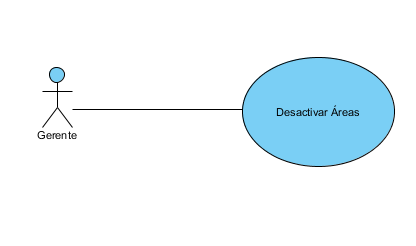
\includegraphics[width=0.8\textwidth]{images/desactivarAreas}
		\caption{Diagrama de Casos de Uso del sistema.}
	\end{figure}
%-------------------------------------- TERMINA descripción del caso de uso.